\documentclass{article}
\usepackage[utf8]{inputenc}
\usepackage{enumitem}
\usepackage{float} % use H for figure placement
\usepackage{pgfplots}
\usetikzlibrary{arrows}
\usepackage{amsmath,amssymb}
\usepackage[margin=1in]{geometry}
\usepackage{hyperref}
\usepackage[amsthm]{ntheorem}
\usepackage{xcolor}
\usepackage{framed}
\definecolor{shadecolor}{rgb}{0.95,0.95,0.95}
\usepackage{physics}

\newtheorem{theorem}{Theorem}[section]
\newtheorem{prop}{Proposition}
\newtheorem{corollary}{Corollary}
\newtheorem{lemma}{Lemma}
\newtheorem{ex}{Example}
\newtheorem*{remark}{Remark}
\theoremstyle{definition}
\newtheorem{definition}{Definition}[section]

\usepackage [autostyle, english = american]{csquotes}
\MakeOuterQuote{"}
\newcommand{\Section}[1]{\hrule\hrule\section{#1}}
\newcommand{\Def}[2]{
\begin{shaded*}
\begin{definition}{\textit{#1}}\\#2\end{definition}
\end{shaded*}
}
\DeclareMathOperator*{\argmin}{arg\,min}
\DeclareMathOperator*{\argmax}{arg\,max}
\def\R{\mathbb{R}}
\def\C{\mathbb{C}}

\title{ENM 521 - MechE Math part 2}
\author{Rebecca Li}
\date{Fall 2019}

\begin{document}
	\maketitle
	\tableofcontents
	
\section*{Organization}
\begin{itemize}
	\item Instructors: Pedro Ponte Castaneda  (Towne 235)
	\item Office Hours: M 4:30-5:30 or by appointment 
	\item TA: Chuanpeng Sun
	\item References: 
	\\\textit{Functions of a complex variable: Theory and Technique}, Carrier. 
	\\\textit{PDE: theory and technique}, Carrier. 
	\\\textit{Introduction to complex variables and Applications}, Churchill. 
	\\\textit{Boundary Value Problems of Mathematical Physics}, Stakgold.

\end{itemize}
\section{Complex Numbers}
Real numbers obey the usual operations. In particular, $\R$ is closed under addition and multiplication. However, there are some operations that are not possible with real numbers:, e.g. Find $x \in \R$ such that $x^2 = -1$.


In addition, there are many mysterious properties of power series:

\begin{remark}
$f(x) = \frac{1}{1+x^2}$ is a nice function. The Taylor series expansion is:
	$$f(x) ~ 1-x^2+x^4+...$$
	
	This diverges for $|x| \geq 1$. Why?
	Even nice functions of a real variables have divergence properties which are related to the fact that for when you generalize to the complex numbers, the function has a singularity at $x=i$.
\end{remark}

\Def{Complex Numbers}{A complex number $z$ is a pair of reals $(x,y):$
$$z = (x,y) \in \C$$
where
$$Re(z) = x \in \R,\ Im(z) = y \in \R$$

This obeys the following:
\begin{itemize}
	\item \underline{Equality:} $z_1 = (x_1, y_1) = (x_2, y_2) \iff x_1 = x_2,\ y_1 = y_2$
	\item \underline{Addition:} $z_1 + z_2 = (x_1 + x_2, y_1+y_2)$
	\item \underline{Multiplication:} $z_1 z_2 = (x_1 x_2 - y_1 y_2, x_1 y_2 + x_2 y_1)$
\end{itemize}
}

Real numbers are a special case of a complex number: $(x, 0) $ "=" $x$. Furthermore, $(1,0)$ is the identity for the reals. 

Similarly, we can define $(0,1)$ to be the complex number $i$ such that:

$$(x,y) = (x, 0) + (0,y) = x + y(0,1) = x + iy$$

In terms of $i$, we can write addition and multiplication:

\begin{itemize}
	\item \underline{Addition:} $z_1 + z_2 = (x_1 + x_2) + i (y_1+y_2)$
	\item \underline{Multiplication:} $z_1 z_2 = (x_1 x_2 - y_1 y_2) + i (x_1 y_2 + x_2 y_1)$
\end{itemize}


\Def{Argand Representation}{We can think of our complex number as a vector in a plane with magnitude $r = |z|$ and angle $\theta = \arg z$. This is such that:

$$\tan \theta = \frac{x}{y}$$

We note that $theta$ is defined up to an arbitrary multiple of $2\pi$ radians. Princple value of $\theta$ such that $-\pi < \theta \leq \pi.$

\begin{figure}[H]
	\centering
	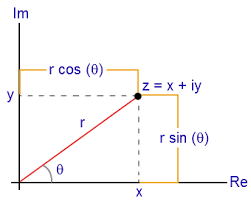
\includegraphics[width=0.5\linewidth]{Argand_plane}
	\caption{The Argand Plane.}
	\label{fig:argand}
\end{figure}
}

\begin{lemma}
	The Triangle Inequality is:
	$$\norm{z_1 + z_2} \leq \norm{z_1} + \norm{z_2}$$
	We can prove this using the argand representation. 
\end{lemma}

Properties of complex numbers:

\begin{itemize}
	\item Commutative
	\item Associative
	\item Distributive
	\item $z_1 -z_2 = z_1 + (-z_2)$.
	\item $z^n = r^n(\cos(n\theta) + i \sin(n\theta)$
	\item Complex Cojugate: $z^* = \bar{z} = x-iy = r(\cos\theta - i \sin\theta)$
	\item $z z^* = \norm{z}^2$
	\item Division 
\end{itemize}

\Def{Roots of Unity}{Given a complex number $z_0$ characterized by $r_0, \theta_0$, can we find a $z$ such that $z^n = z_0$? Well, clearly:
$$r^n = r_0$$
$$\cos(n\theta) + i \sin(n\theta) = \cos(\theta_0) + i \sin(n\theta_0)$$

This, $\norm{z} = r_0^{1/n}$, and $n\theta = \theta_0 + 2k\pi,\ k = 0, \pm 1, \pm 2...)$ There are only $n$ different solutions, meaning there are only $n$ roots. If we let $z_0 = 0$, we can find the roots of unity:

$$\text{roots of unity} = z = \cos(\frac{2k\pi}{n}) + i \sin(\frac{2k\pi}{n})$$
If we let $\omega = \cos(\frac{2\pi}{n}) + i \sin(\frac{2\pi}{n})$, then $\sum_{k=0}^{n-1} \omega^k = 0$

TODO: rebecca, this seems a bit wrong. See \href{https://en.wikipedia.org/wiki/Root_of_unity}{https://en.wikipedia.org/wiki/Root\_of\_unity} for a better explanation.

Essentially, geometrically, this means that the powers of $\omega$ sum to zero, as in Figure \ref{fig:3rdrootsofunity}.

\begin{figure}[H]
	\centering
	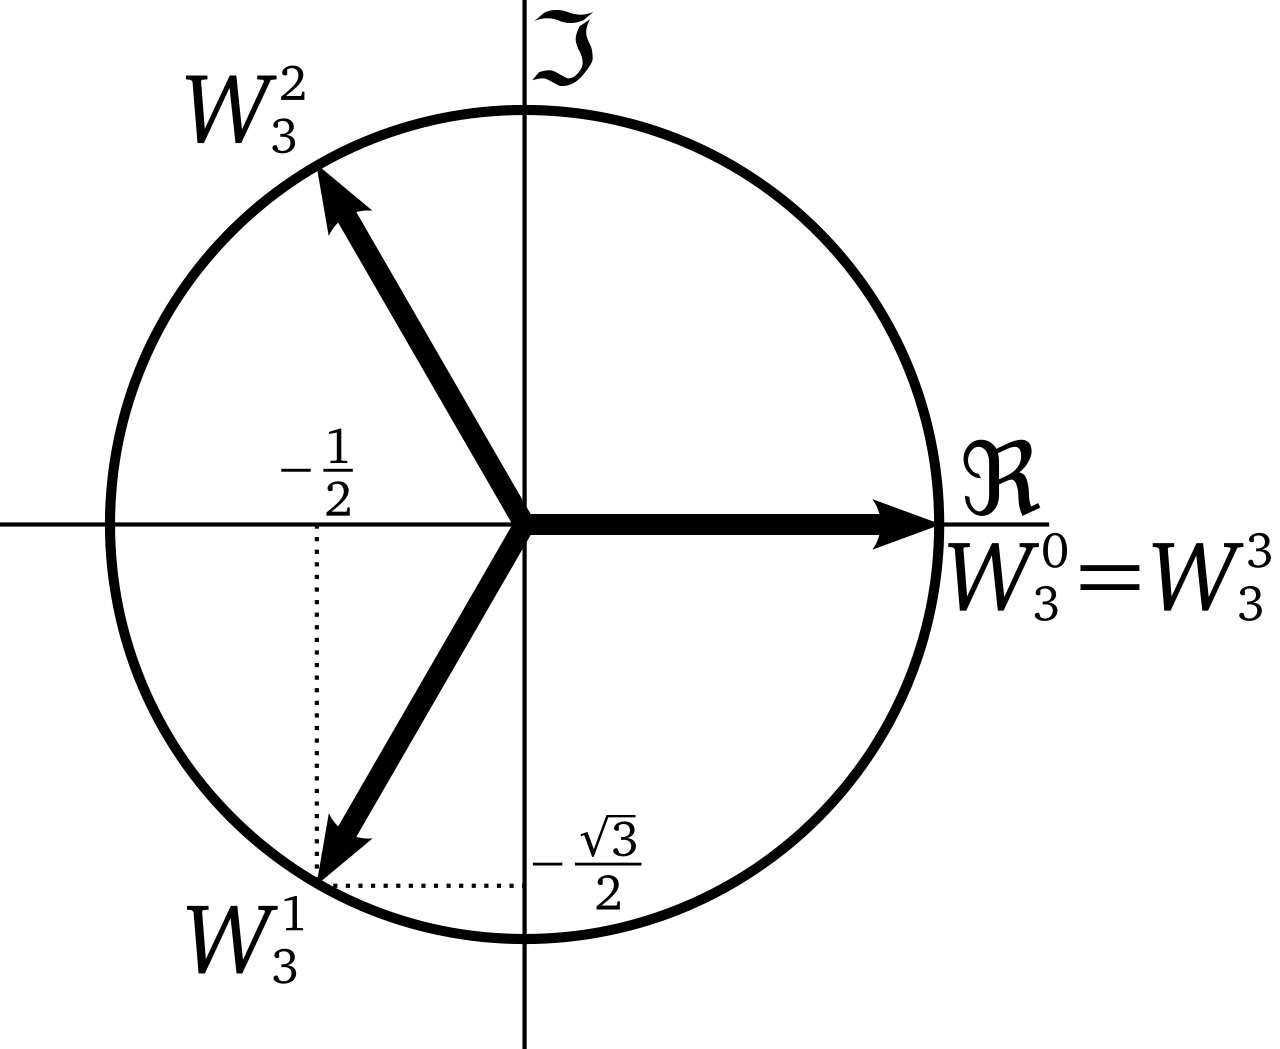
\includegraphics[width=0.5\linewidth]{3rd_roots_of_unity}
	\caption{The third roots of unity sum to one - as do nth roots of unity. \textit{Wikipedia.}}
	\label{fig:3rdrootsofunity}
\end{figure}

}

The complex numbers lack the notion of order, in the way the real numbers have order. In particular, the notion of $\infty$ is very different. For real numbers, we have $\pm \infty$, which serves as an upper and lower bound on $\R$. For complex numbers, we define a \textit{point at infinity}. The point at infinity is the limit of what happens as $r$ goes to infinity for $z=r e^{i\theta}$, While it may seem like this goes to a different point for different $\theta$, the point at infinity is in fact the same.

One way to imagine this is to consider the \textit{stereographic projection} (Figure \ref{fig:stereographic}):
\begin{figure}[H]
	\centering
	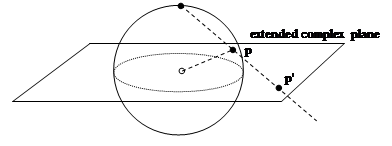
\includegraphics[width=0.5\linewidth]{stereographic_projection}
	\caption{The stereographic projection. We can see that as the point picked to move away from the point at infinity (the north pole), becomes horizontal. The intersection point on the sphere will gradually move closer to the point at the north pole, hence the north pole is the point at infinity. \textit{MathPages}.}
	\label{fig:stereographic}
\end{figure}


\section{Real and imaginary pairs of Z}

\begin{align}
	f(z) = u(x,y)+iv(x,y)
\end{align}

The continuity of $f(z)$ is continuous at $z = x_0 + iy_0$ $\iff u(x,y)$ and $v(x,y)$ are continuous at $x_0, y_0$ 

\subsection{Differentiation of complex functions}

\Def{Differentiable}{A function $f$ is differentiable at point $z$ if 
\begin{itemize}
	\item $\lim_{h\to0} \frac{f(z+h) - f(z)}{h} = f'(z)$ exists
\end{itemize}

\textbf{Note:} $h \in \C$ and can approach zero along any path. 
}


\begin{ex}
$f(z) = z^2$ is everywhere differentiable. 
\end{ex}

\begin{ex}
	$f(z) = |z|$ is continuous, but not differentiable at $z = 0$. 
	
	If we look at the definition:
	
	$\lim_{h\to0} \frac{f(z+h) - f(z)}{h} = \lim \frac{|h|}{h}$
	
	but $|h|$ approaches 0 so the limit does not exist.
\end{ex}



\begin{theorem}
	Differential of a Complex function
\begin{enumerate}
	\item If $f(z) = z^m$, m is integer, then $f'(z) = mz^{m-1}$
\end{enumerate}
If $f(z)$ and $g(z)$ are differentiable, then:
\begin{enumerate}
	\item$(f+g)' = f'+g'$
	\item$(fg)' = f'g + fg'$
	\item$(f/g)' = \frac{f'g-fg'}{g^2},\ g \neq 0 $
\end{enumerate}


Suppose g is differentiable at z and f is differentiable at g(z). If F(z)=f(g(z)), then:

$$ F'(z) = f'(g(z))g'(z)$$

Suppose that $h \to 0$ along the real axis. Then:

\begin{align}
\frac{f(z+h) - f(z)}{h} & = \frac{u(x+h, y) + iv(x+h,y) - u(x,y) - iv(x,y)}{h}\\
& = \frac{u(x+h, y) - u(x,y) }{h} + i \frac{v(x+h,y) v(x,y)}{h}
\end{align}

If f is differentiable at z = x+iy, both limits (as $h \to 0$) must exist and:

$$f'(z) = \frac{\partial u}{\partial x} + i  \frac{\partial v}{\partial x}$$

Next, suppose that h = ik, $k \in \R$.

\begin{align}
\frac{f(z+h) - f(z)}{h} & = \frac{u(x, y+k) + iv(x,y+k) - u(x,y) - iv(x,y)}{ik}\\
& = \frac{u(x, y+k) - u(x,y) }{ik} + i \frac{v(x,y+k) v(x,y)}{ik}
\end{align}

Since f is differentiable, both limits as $k \to 0$ must exist. We can conclude that:

$$f'(z) = \frac{\partial v}{\partial y} - i  \frac{\partial u}{\partial y}$$

We conclude that:


$$\boxed{f'(z) = \frac{\partial u}{\partial x} + i  \frac{\partial v}{\partial x} = \frac{\partial v}{\partial y} - i  \frac{\partial u}{\partial y}}$$


We can additionally conclude the \textbf{Cauchy-Riemann Conditions}:

$$\frac{\partial u}{\partial x} = \frac{\partial v}{\partial y},\ \frac{\partial v}{\partial x} = -\frac{\partial u}{\partial y}$$

\end{theorem}

\Def{Cauchy-Riemann Equations}{For a function $f(z) = u(x,y)+iv(x,y)$:
	$$\frac{\partial u}{\partial x} = \frac{\partial v}{\partial y},\ \frac{\partial v}{\partial x} = -\frac{\partial u}{\partial y}$$
	
	These furnish a necessary condition for differentiability at a point.
	
	\begin{remark}
		The Cauchy-Riemann equations are necessary, but \textbf{not} sufficient for differentiability at a point.
\end{remark}}

\begin{ex} Consider the complex conjugate function:
	$$f(z) = z^* = \bar{z} = x-iy$$
	
	We would like to determine if $f$ is differentiable. If it is, it must satisfy Cauchy-Riemann equations.
	
	$$\frac{\partial u}{\partial x} = 1,\ \frac{\partial v}{\partial y} = -1$$
	
	Already, we see that $\frac{\partial u}{\partial x} \neq \frac{\partial v}{\partial y}$. So $f(z)$ is not differentiable for any value of z.
\end{ex}

\begin{remark}
The Cauchy-Riemann equations can also be written as:

$$f'(z) = \frac{\partial f}{\partial x} = -i \frac{\partial f}{\partial y}$$

\end{remark}


\begin{theorem}
	Let $f=u+iv$ be differentiable with complex partials at $z=re^{i\theta}$. Then:
	$$\pdv{u}{r} = \frac{1}{r} \pdv{v}{\theta},\ \pdv{v}{r} = -\frac{1}{r} \pdv{u}{\theta}$$
\end{theorem}


\Def{Analyticity}{A function is \textbf{analytic (holomorphic) }at a point if it is differentiable everywhere in some neighborhood of the point. If the function is analytic for all values of $z \in \C$, then it is \textbf{entire}. 
	
Note: Being differentiable in a neighborhood (analytic) is a stronger requirement than just differentiable. 

\textbf{Remark:} If a function is analytic at a point, it is differentiable for all orders at that point.
}


\begin{ex} Let 
$f(z) = |z|^2 = z \bar{z}$. This function is differentiable only at $z=0$, but it is nowhere analytic. 
\end{ex}

\begin{theorem}Let $f(z) = u(x,y)+iv(x,y)$  be defined in a domain D. Let $u(x,y)$ and $v(x,y)$ have continuous partials that satisfy Cauchy-Riemann equations for all points in D. Then, we can show that $f(z)$ is analytic in D. Thus, Cauchy-Riemann applied to the neighborhood is sufficient to show analyticity.
\end{theorem}

\begin{ex}
$f(z)=e^z = e^z=e^x(\cos y + i \sin y)$


Therefore, $e^z$ is an entire function. 

$$f'(z) = e^z$$
\end{ex}

Note: if $f$ is analytic of non-zero at a point z, then a branch may be chosen for which $\log (f(z))$ is also analytic in the neighborhood of z and $\dv{}{z} log(f(z)) = \frac{f'(z)}{f(z)}$


\section{Branch points and Branch Cuts}
Explaining the epsilon method: \url{https://math.stackexchange.com/questions/2150639/branch-point-of-logz}
The easy way to do branch points is to remember that $log(z)$ and $z^p$ where p is non integer both have branch points at $0, \infty$. So simply find when $z = 0, \infty$ for those functions to get the branch points. Then a branch cut must connect all branch points, but does not have to go in any particular way. For $log(z)$, the negative real line is often the branch cut that is picked.




\section{Harmonic functions}
Later, we will see that analytic functions have derivatives of all orders. Recall:
$$f'(z) = \frac{\partial f}{\partial x} = -i \frac{\partial f}{\partial y}$$

We can take the derivative:

$$f''(z) = \frac{\partial f}{\partial x} = -i \frac{\partial f}{\partial y}$$
And so:
$$\pdv{^2f}{x^2} + \pdv{^2f}{y^2} = 0$$

Since $f(z) = u(x,y) + i v(x,y)$, 

$$\pdv{^2u}{x^2} + \pdv{^2u}{y^2} = 0 \pdv{^2v}{x^2} + \pdv{^2v}{y^2} = 0$$

\Def{Harmonic Function}{ A continuous, real valued function u(x,y) defined on domain D is called \textbf{harmonic} if it has continuous first and second derivatives, satisfying Laplace's equation:
$$\pdv{^2u}{x^2} + \pdv{^2u}{y^2} = 0$$ 

Note: The real and imaginary parts of an analytic functions are harmonic functions.}

\Def{Harmonic Conjugate}{If $f(z) = u + iv$ is analytic, $v$ is called the harmonic conjugate of $u$, and vice versa.}

\begin{remark}
Laplace's equation furnishes a \textbf{necessary} condition for a function to be real and imaginary parts of an analytic function.
\end{remark}

\begin{ex}
$u(x,y) = x^2+y$

This cannot be the real part of any analytic function, since the Laplace equations are not satisfied. $$\pdv{^2u}{x^2} + \pdv{^2u}{y^2} \neq 0 $$.
\end{ex}

\section{Sequences}
\Def{Sequence}{ A sequence $\{z_n\}$ of complex numbers is an assignment of a complex number $z_n$ to each positive integer $n$.}

\Def{Convergent sequence}{A sequence $\{z_n\}$ is said to have a limit $z_0$ or converge to $z_0$ which we write as 

$$\lim_{n\to\infty} z_n = z_0$$

if for every $\epsilon > 0, \exists\ M \in  \mathbb{Z}$, such that:

$$|z_n - z_0| < \epsilon,\ \forall n > M$$

This means for sufficiently large values of $n$, $z_n$ is arbitrarily close to $z_0$.

\begin{figure}[H]
	\centering
	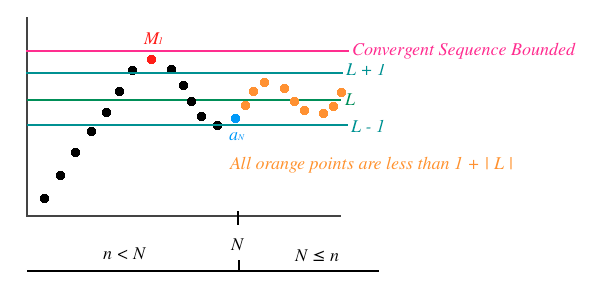
\includegraphics[width=0.7\linewidth]{convseq}
	\caption{A convergent sequence example. }
	\label{fig:convseq}
\end{figure}

Alternative definition: Every neighborhood of $z_0$ contains all but a finite number of $z_n$'s.
}

\begin{ex}
$\{\frac{1}{m}\}$ converges to 0. However, $\{(-1)^{m}\}$ does not converge. 
\end{ex}

\begin{theorem}
Let $z_m = x_m + i y_m$ be a sequence of complex numbers $\{z_m\}$. Then, this converges to $z_0 = x_0 + i y_0$ if and only if the real sequences $\{x_m\}, \{y_m\}$ converge to $x_0, y_0$ respectively.

\textbf{Remark}: The properties of complex sequences can be derived from corresponding properties of real sequences. For example, the uniqueness of the limit (can only converge to one value).
\end{theorem}

\begin{theorem}
A convergent sequence is bounded. 

\textbf{Proof:}

If $\lim_{m\to\infty}z_m = z_0$, then there must be a $z_m \in N(z_0,1)$ , where $N$ means neighborhood, for $m>N$, let $M = \max\{|z_1|, .., |z_N|\}$, then
$$|z_m| < M + |z_0| + 1, \forall m$$

Note that the converse is not true. Counterexample:

$\{1,2,1,2,1,2\}$ is bounded but does not converge. 
\end{theorem}
\Def{Subsequence}{A subsequence of $\{z_m\}$ is a sequence $\{z_{m_k}\}$ whose terms are selected from the terms in an original sequence and arranged in the same order. Subsequences may converge even if sequences do not.}
\begin{ex}
Given a sequence $z_m = (-1)^{m}$, a subsequence could be $z_{m_k} = z_{2k}$, or the even terms, which results in $\{1,1,..1\}$ which converges to 1. The subsequence $z_{m_k} = z_{2k+1}$ converges to -1.
\end{ex}

\begin{theorem}
If a sequence $\{z_m\}$ converges to $z_0$, then every subsequence also converges to $z_0$. 
\end{theorem}

\begin{theorem}
Every bounded sequence of complex numbers contains at least one convergent subsequence. 

\textbf{Proof:} Exercise. 
\end{theorem}

\Def{Cauchy Sequence}{A sequence is Cauchy sequence if in the limit, the difference between the terms becomes arbitrarily small (each value becomes arbitrarily close to each other), which lets us not define the actual limit. 

Formally, a sequence $\{z_m\}$ of complex numbers is a Cauchy sequence if for every $\epsilon>0$, $\exists N \in \mathbb{Z}$ such that $|z_m - z_M| < \epsilon,\ \forall m, M>N$.}

\begin{theorem}
A sequence $\{z_m\}$ converges if and only if $\{z_m\}$ is a Cauchy sequence. 

Note: The two notions of convergence and Cauchy convergence are equivalent. Cauchy convergence is the most general test of convergence. It works even if the limit $z_0$ is not known.
\end{theorem}

\section{Series}
\Def{Series}{Given a complex sequence $\{a_m\}$, we associate a new sequence defined by $s_m = \sum_{k=1}^{n}a_k$. Then, we say that $\sum_{k=1}^{\infty}a_k$ is a series. The series is said to converge or diverge according to whether the sequence $\{s_m\}$ converges or diverges. We call $\{s_m\}$ the \textbf{partial sum} of the series, and $a_k$ the kth term.

\textbf{Note:} Every theorem about sequences can be rephrased to be a theorem about series, since series are sequences, and vice versa
}
\begin{theorem}
Let $\{a_m\}$ be a sequence of complex numbers, with $a_m = \alpha_m+ i \beta_m$ where $\{\alpha_m\}, \{\beta_m\}$ are sequences of real numbers. Then, by the earlier result, the complex series $\sum_{k=1}^{\infty}a_k$ converges if and only if $\sum_{k=1}^{\infty}\alpha_k$ and $\sum_{k=1}^{\infty}\beta_k$ converge.
\end{theorem}


\Def{Cauchy Criterion.}{Let $s_m = \sum_{k=1}^{m}a_k$. The series $\sum_{k=1}^{\infty}a_k$ converges if and only if for every $\epsilon>0$, there exists $N \in \mathbb{Z}$ for $m, M>N$:

$$|s_M - s_m| = \left|\sum_{k=m+1}^{M}a_k\right| < \epsilon$$

Alternatively, letting $M = m+p$:

$$|s_{m+p} - s_m| = \left|\sum_{k=m+1}^{m+p}a_k\right| < \epsilon, \forall p = 1,2,3,..$$

This is the most general test for convergence of a series. 

Note: Familiar properties of a series are immediate consequences of the Cauchy criterion.

Note: $a_k \to 0$ to converge. (set $p=1$).
 }

\Def{Absolutely Convergence}{A series $\sum_{m=1}^{\infty}a_m$ is said to be absolutely convergent if $\sum_{m=1}^{\infty}|a_m|$ converges. 

\textbf{Note:} Applying the triangle inequality:

$$\left|\sum_{k=m+1}^{m+p}a_k\right| \leq \sum_{k=m+1}^{m+p}\left|a_k\right|$$

Applying this with the Cauchy criterion, we can deduce that absolute convergence of a series ensures its convergence. 

\textbf{Note:} If $|a_m| \leq |b_m|$, for every $m$, the convergence of $\sum_{m=1}^{\infty} |b_m|$ implies convergence of $\sum_{m=1}^{\infty} |a_m|$ .
}

\begin{theorem}
Suppose $a_m>0\ \forall m$ and that $\sum_{m=1}^{\infty} a_m$ diverges. If $s_m = \sum_{k=1}^m a_k$, then:
\begin{enumerate}
	\item $\sum_{m=1}^{\infty} \frac{a_m}{s_m}$ also diverges.
	\item $\sum_{m=1}^{\infty} \frac{a_m}{s_m^2}$ also converges. This is shown by Cauchy. 
\end{enumerate}
\end{theorem}

\begin{corollary}
The series 	$\sum_{m=1}^{\infty} \frac{1}{m}$ also diverges. But $\sum_{m=1}^{\infty} \frac{1}{m^2}$ converges.
\end{corollary}

\begin{theorem}Geometric series
Consider $s_m = \sum_{k=1}^m r^{k-1} = \frac{1-r^m}{1-r}$. This is a geometric series.  

\textbf{Proof:}

\begin{align}
(1-r)\sum_{k=1}^m r^{k-1} &= \sum_{k=1}^m r^{k-1} - r-^k \\ 	
& = 1-r^m
\end{align}

Hence a series $\sum_{m=1}^\infty a_m$ converges absolutely if ther eexists a constant $r \in [0,1)$ and a real number M such that $|a_m| < M r^m,\ m>M$
\end{theorem}

\end{document}